\section{Proposed Mechanism}

\subsection{Using 6top Transaction}
\begin{withoutheadline}
\begin{frame}{Using 6top Transaction}


\setbeamercolor{block title}{bg=blue!30,fg=black}
\setbeamercolor{block body}{bg=blue!10,fg=black}
\setbeamertemplate{blocks}[rounded][shadow=false]

\begin{block}{Why?}
    \begin{itemize}
    \item  Submitted in the shared slot.
    \item<2-> Contains the reserved cells.
    \end{itemize}
    \end{block}

\only<3->{
\begin{block}{How?}
    \begin{itemize}
    \item<3-> The child node Sends an Add Request.
    \item<4-> The parent replies with the selected cells.
    \item<5-> The Neighbor nodes collects the reserved cells and save them. 
    \end{itemize}
    \end{block}}
    
    
\begin{figure}[p]

 
  \only<3>{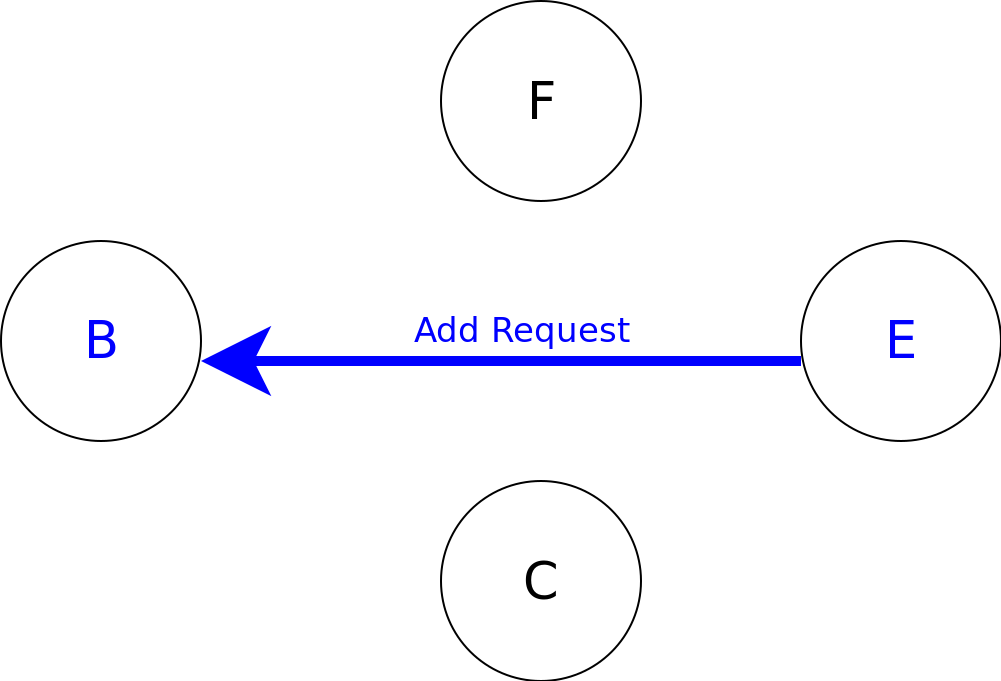
\includegraphics[width=.4\linewidth]{figures/usin1.png}}
  \only<4>{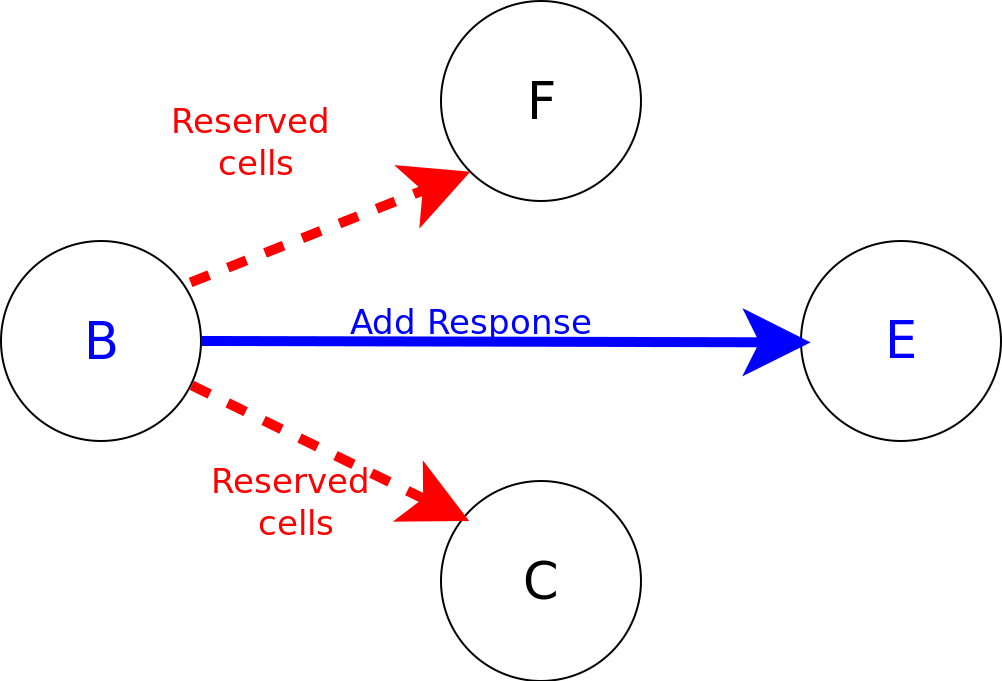
\includegraphics[width=.4\linewidth]{figures/usin2.png}}
  \only<5>{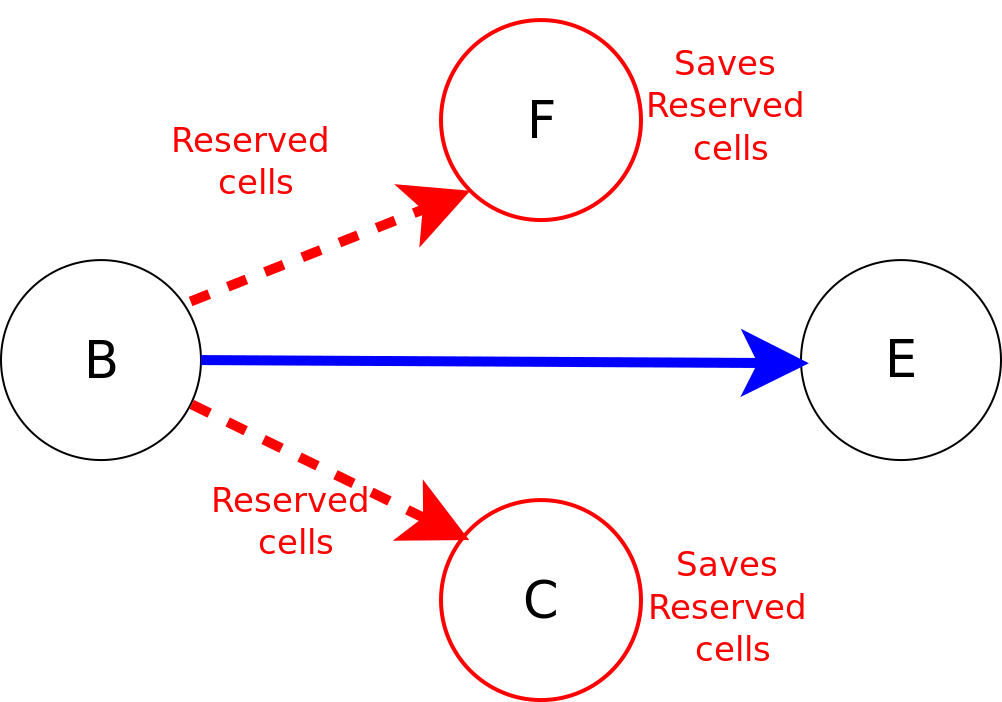
\includegraphics[width=.4\linewidth]{figures/usin3.png}}
\end{figure}

\end{frame}
\end{withoutheadline}

\subsection{Avoid Table}



\begin{withoutheadline}
\begin{frame}{Avoid Table structure and functioning}


\setbeamercolor{block title}{bg=blue!30,fg=black}
\setbeamercolor{block body}{bg=blue!10,fg=black}
\setbeamertemplate{blocks}[rounded][shadow=false]
\begin{block}{Avoid Table}
    \begin{itemize}
     \item The cells reserved by neighbors will be saved by a structure similar to TSCH table. 
    \item<2-> Scheduling function will avoid selecting cells found in this structure. 
    \item<3-> 6top will manage this table.
    \end{itemize}
    \end{block}
    
    
\begin{figure}[p]

 
  \only<1>{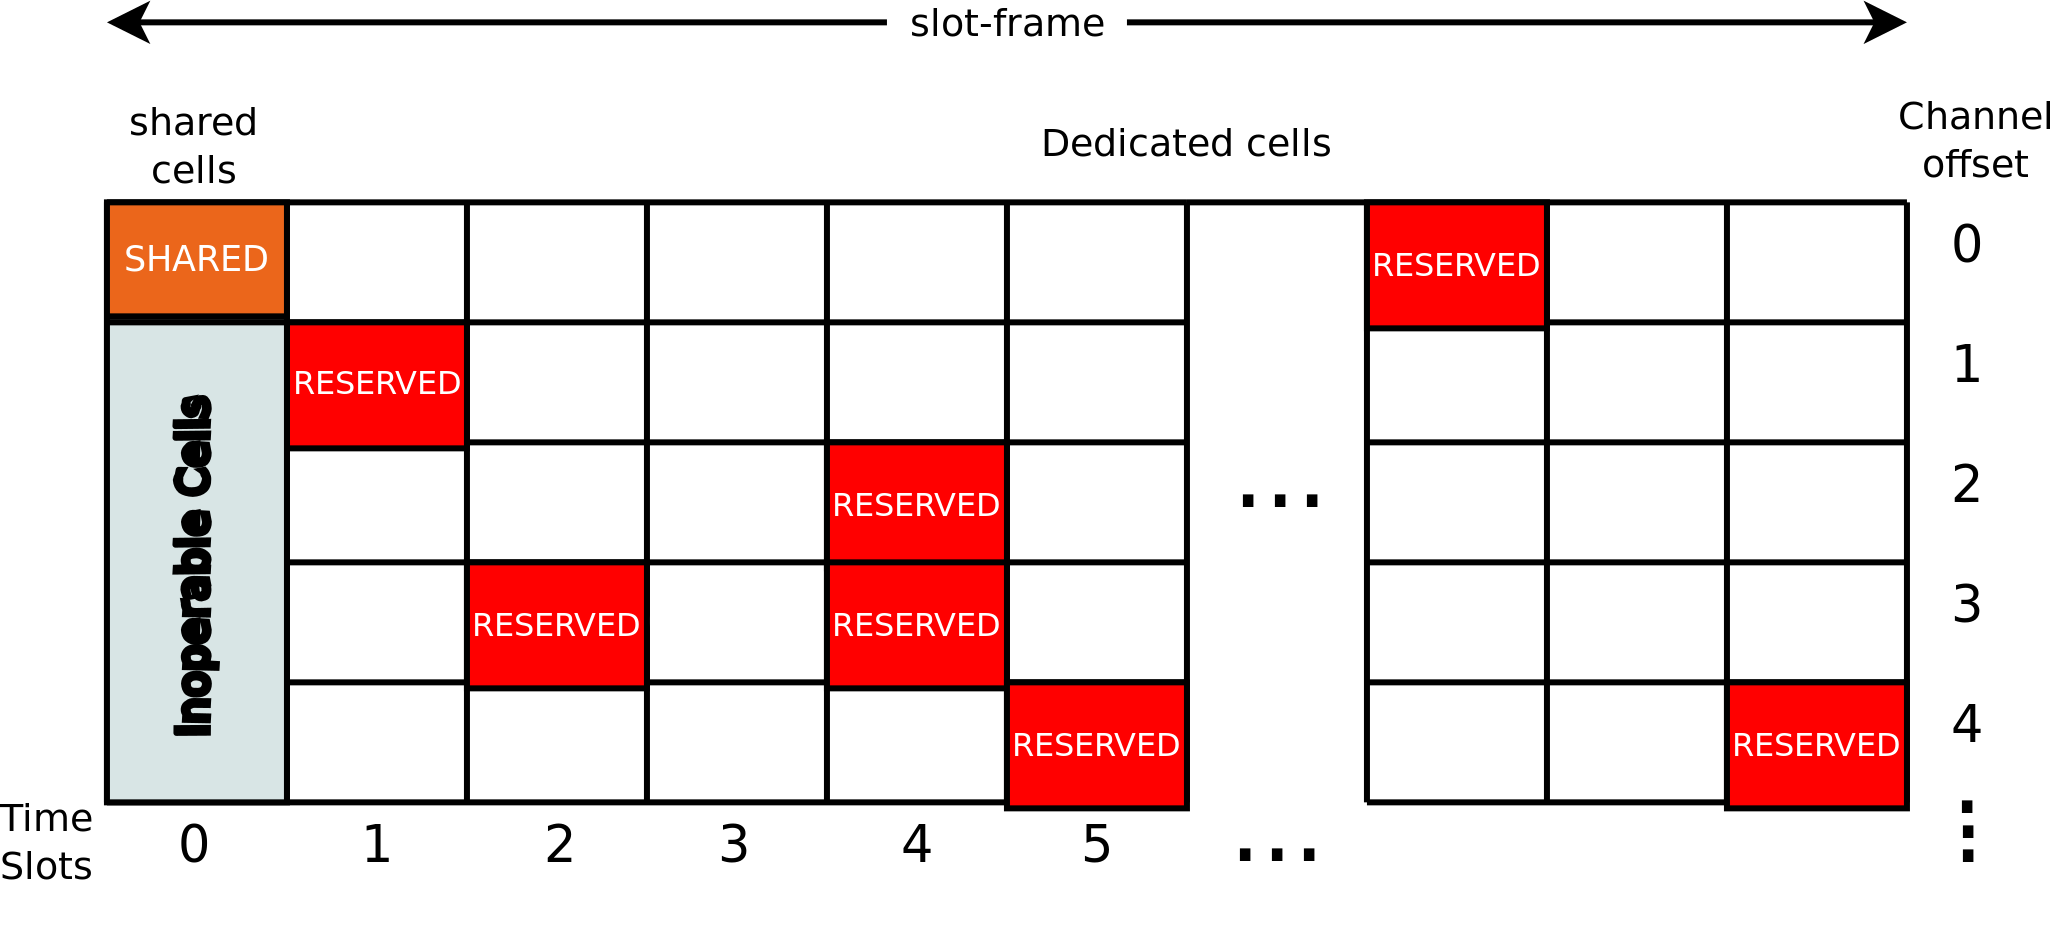
\includegraphics[width=.8\linewidth]{figures/avoid.png}}
  \only<2->{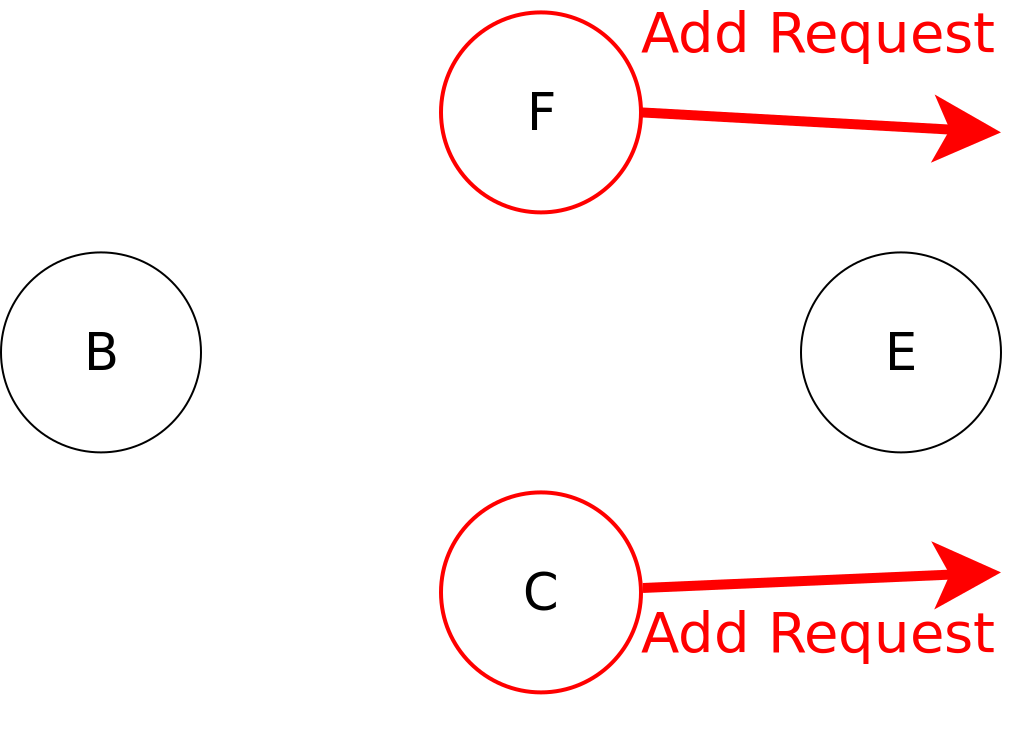
\includegraphics[width=.4\linewidth]{figures/avoid2.png}}
 
\end{figure}



\end{frame}
\end{withoutheadline}


\subsection{Cell Buffer}
%% edit 
\begin{withoutheadline}
\begin{frame}{Cell Buffer}

\begin{itemize}
    \item We have created a probablistic model to calaculate the optimal length of the buffer.
    \item<2-> $p$ is the probability of successful transmission.
    \item<3-> we are confidence with a probability $P_{o}$ that one of the transmission is successful.
    \item<4-> $k$ is the number of retransmission (the optimal length of the buffer). 
    \item<5-> we end up with the following equation using binomial distribution:
    
    \end{itemize}
    
 \centering
\begin{figure}[p]

\item<5-> 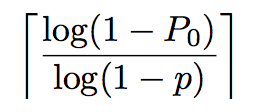
\includegraphics[width=0.3\linewidth]{figures/9nq6n.png}
\end{figure}
\begin{itemize}
\item<6-> According to this equation, and by taking the worst case scenario a buffer of length 10 can assure us 95\% of success
 \end{itemize}
\end{frame}
\end{withoutheadline}